%-*- coding: utf-8 -*-
\textcolor[RGB]{46, 116, 181}{\chapter{Initialisation}}
Quelle que soit l’importance des avancées scientifiques et technologiques, c’est le travail des
professionnels de santé qui détermine la qualité et l’efficacité des soins. Dans ce contexte, les soins
nutritionnels, qui portent sur l’évaluation de l’état nutritionnel et l’accompagnement alimentaire des
patients hospitalisés, en interaction étroite avec l’équipe de soin, ne font pas exception. Pour ce
faire, les diététiciens développent des actions de complexité variable, tant au niveau des services de
soins que du système de restauration.

Simultanément, les professionnels doivent faire face à de nouveaux défis, dus aux modifications des
profils épidémiologiques, démographiques et sociaux des populations, ce qui exige la mise en place
de nouvelles compétences et la reconfiguration des stratégies d’action. Pour les diététiciens du
secteur hospitalier, elles ont pour conséquences de nouvelles exigences mentales et surtout
cognitives.

Le niveau de développement industriel de la filière alimentaire française allège la charge de travail
technique des diététiciens, non seulement en ce qui concerne la diversité de matières premières,
mais également dans le domaine du contrôle \enquote{qualité}, tout au long de la chaîne de production. De
la même façon, les nouveaux concepts de production en restauration collective, caractérisés par
l’utilisation de produits pré élaborés et l’innovation technologique des équipements, gagnent
visiblement du terrain dans le secteur hospitalier français.

\section{Définition du problème}
L'élaboration de menus dans un hôpital pour la restauration des patients
est une tâche complexe, et doit tenir compte des différentes pathologies
rencontrées. Faute de moyens (temps et argent) seules quelques grandes
lignes de restauration sont retenues; alors qu'idéalement, chaque
patient devrait pourvoir avoir un repas adapté à sa pathologie.

\section{Vision du projet}
\subsection{Solution envisagée}
Le projet Vitameal a pour objectif de faire correspondre au mieux la planification des régimes et des
prescriptions diététiques aux repas réellement servis au patient. Il consiste en un outil interfaçant la
gestion de production, la prise de commande et le suivi nutritionnel des repas.

\subsection{Périmètre}
C'est un diététicien qui renseigne le profil diététique des patients,
sous les directives des médecins. C'est aussi un diététicien qui élabore
les menus des patients. L'outil élaborera donc
les menus par filtrage des produits correspondants aux profils
diététiques des patients. Pour des raisons de simplifications, nous nous limiterons dans ce projet aux seuls patients adolescents et adultes, à l'exclusion des personnes agées.
\begin{figure}[H]
\label{Modelisation_du _probleme}
  \centering
      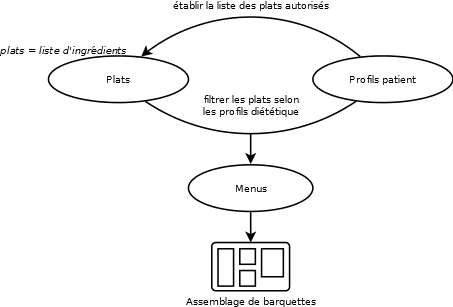
\includegraphics[width=0.75\textwidth]{problem_model} %
\caption{Modélisation du problème}
\end{figure}

\section{Analyse des exigences}
\subsection{Partie prenantes}
\begin{itemize}
\item Participantes~: les diététiciens, le service restauration
\item Concernés~: les médecins, la direction (budget)
\item Impactées~: les patients
\end{itemize}

\subsection{Les besoins}
\begin{description}
\item[] En tant que diététicien, j’ai besoin de :
\begin{description}
 \item[N001:] pouvoir renseigner le profil diététique des patients, afin qu’ils
 puissent bénéficier de menus adaptés.
 \item[N002:] pouvoir élaborer les menus des 3 repas journaliers
 (petit-déjeuner, déjeuner et dîner dont la composition est décrite en annexe
 \ref{annexeA}), de façon automatique, en tenant compte de grammages dépendant du type d'aliments et de la tranche d'age (Document \ref{docNutrition}, Annexe 2).
 \item[N003:] pouvoir saisir des plats et leur composition.
 \item[N004:] élaborer des menus selon les fréquences de service, selon le
 document \ref{docNutrition}, Annexe 4.
 \item[N005:] classer chaque aliment dans une des catégories d’aliments citée
 dans les tables de grammages du document \ref{docNutrition}, Annexes 2 et 4.
\end{description}
\item[N006:] En tant qu’administrateur du site internet de l’hôpital, j’ai
besoin de récupérer le menu de la semaine, afin pouvoir l’intégrer au site.
\item[N007:] En tant que médecin, j’ai besoin de consulter les profils
diététiques des patients admis, pour les  valider.
\item[N008:] En tant que cuisinier du service restauration, j’ai besoin de
consulter les menus élaborés, afin de pouvoir les préparer et prévoir les ingrédients à commander.
\item[N009:] En tant qu’agent de restauration hospitalière,  j’ai besoin de
connaître les menus de chaque patient, afin de pouvoir assembler les plateaux repas.
\end{description}
\subsection{Les contraintes}
\begin{description}
\item[N010:] Les médecins doivent pouvoir vérifier / valider les profils
diététiques des patients.
\item[N011:] La direction fixe un budget maximum par menu.
\end{description}

\subsection{Exigences}

\rowcolors{1}{}{}

\begin{table}[!h]

\begin{tabular}{|p{60mm}p{100mm}|}

\hline

\multicolumn{2}{|l|}{\textbf{REQ\_0100:} 3 repas} \\ \hline

\emph{Type:} Métier & \emph{Liens:} REQ\_0101 REQ\_0105  \\

\emph{Origine:}  & \emph{Validé:} Non \\

\emph{Version:} Initial & \emph{Test:}  \\

\emph{Priorité:} Must & \\ \hline

\multicolumn{2}{|p{16cm}|}{Le système doit permettre de concevoir les 3 repas (petit-déjeuner, déjeuner, souper) d'une journée.} \\ \hline

\end{tabular}

\end{table}



\begin{table}[!h]

\begin{tabular}{|p{60mm}p{100mm}|}

\hline

\multicolumn{2}{|l|}{\textbf{REQ\_0101:} Petit déjeuner} \\ \hline

\emph{Type:} Métier & \emph{Liens:} REQ\_0102 REQ\_0103 REQ\_0104  \\

\emph{Origine:}  & \emph{Validé:} Non \\

\emph{Version:} Initial & \emph{Test:}  \\

\emph{Priorité:} Should & \\ \hline

\multicolumn{2}{|p{16cm}|}{Le système doit permettre de concevoir un petit-déjeuner composé d'une boisson, d'un aliment céréalier, d'un produit laitier et d'un fruit.} \\ \hline

\end{tabular}

\end{table}



\begin{table}[!h]

\begin{tabular}{|p{60mm}p{100mm}|}

\hline

\multicolumn{2}{|l|}{\textbf{REQ\_0102:} Éléments petit déjeuner} \\ \hline

\emph{Type:} Métier & \emph{Liens:}  \\

\emph{Origine:}  & \emph{Validé:} Non \\

\emph{Version:} Initial & \emph{Test:}  \\

\emph{Priorité:} Must & \\ \hline

\multicolumn{2}{|p{16cm}|}{Le système doit permettre de rajouter au petit déjeuner un élément lipidique, sucré ou protodique.} \\ \hline

\end{tabular}

\end{table}



\begin{table}[!h]

\begin{tabular}{|p{60mm}p{100mm}|}

\hline

\multicolumn{2}{|l|}{\textbf{REQ\_0103:} Éléments non diététiques} \\ \hline

\emph{Type:} Métier & \emph{Liens:}  \\

\emph{Origine:}  & \emph{Validé:} Non \\

\emph{Version:} Initial & \emph{Test:}  \\

\emph{Priorité:} Should & \\ \hline

\multicolumn{2}{|p{16cm}|}{Le système doit avertir l'utilisateur de l'usage d'élément non diététique dans un petit déjeuner.} \\ \hline

\end{tabular}

\end{table}



\begin{table}[!h]

\begin{tabular}{|p{60mm}p{100mm}|}

\hline

\multicolumn{2}{|l|}{\textbf{REQ\_0104:} Fréquence éléments non diététiques} \\ \hline

\emph{Type:} Métier & \emph{Liens:}  \\

\emph{Origine:}  & \emph{Validé:} Non \\

\emph{Version:} Initial & \emph{Test:}  \\

\emph{Priorité:} Should & \\ \hline

\multicolumn{2}{|p{16cm}|}{Le système doit vérifier que la fréquence de l'usage d'élément non diététique des petits déjeuners ne dépasse pas 3 repas sur 20, il avertit l'utilisateur si c'est le cas.} \\ \hline

\end{tabular}

\end{table}



\begin{table}[!h]

\begin{tabular}{|p{60mm}p{100mm}|}

\hline

\multicolumn{2}{|l|}{\textbf{REQ\_0105:} Composition déjeuner} \\ \hline

\emph{Type:} Métier & \emph{Liens:}  \\

\emph{Origine:}  & \emph{Validé:} Non \\

\emph{Version:} Initial & \emph{Test:}  \\

\emph{Priorité:} Must & \\ \hline

\multicolumn{2}{|p{16cm}|}{Le système de concevoir un déjeuner et souper composés de 4 ou cinq composantes parmi : entrée, plat protodique, garniture, produit, laitier desserts + de l'eau et du pain (selon le tableau sur la composition du déjeuner en annexe A).} \\ \hline

\end{tabular}

\end{table}



\begin{table}[!h]

\begin{tabular}{|p{60mm}p{100mm}|}

\hline

\multicolumn{2}{|l|}{\textbf{REQ\_0106:} Ajout de plats} \\ \hline

\emph{Type:} Métier & \emph{Liens:}  \\

\emph{Origine:}  & \emph{Validé:} Non \\

\emph{Version:} Initial & \emph{Test:}  \\

\emph{Priorité:} Must & \\ \hline

\multicolumn{2}{|p{16cm}|}{Le système doit permettre d'ajouter des plats et leur définition dans la listes des plats pouvant être préparés.} \\ \hline

\end{tabular}

\end{table}



\begin{table}[!h]

\begin{tabular}{|p{60mm}p{100mm}|}

\hline

\multicolumn{2}{|l|}{\textbf{REQ\_0107:} Description d'un plat} \\ \hline

\emph{Type:} Métier & \emph{Liens:}  \\

\emph{Origine:}  & \emph{Validé:} Non \\

\emph{Version:} Initial & \emph{Test:}  \\

\emph{Priorité:} Must & \\ \hline

\multicolumn{2}{|p{16cm}|}{Le système doit permettre la description d'un plat avec sa liste d'ingrédients et les quantités nécessaires à sa réalisation.} \\ \hline

\end{tabular}

\end{table}



\begin{table}[!h]

\begin{tabular}{|p{60mm}p{100mm}|}

\hline

\multicolumn{2}{|l|}{\textbf{REQ\_0108:} Fréquence de service} \\ \hline

\emph{Type:} Métier & \emph{Liens:}  \\

\emph{Origine:}  & \emph{Validé:} Non \\

\emph{Version:} Initial & \emph{Test:}  \\

\emph{Priorité:} Must & \\ \hline

\multicolumn{2}{|p{16cm}|}{Le système doit proposer un plat selon la fréquence de service de ce plat (exemple 4 fois tous les 20 repas).} \\ \hline

\end{tabular}

\end{table}



\begin{table}[!h]

\begin{tabular}{|p{60mm}p{100mm}|}

\hline

\multicolumn{2}{|l|}{\textbf{REQ\_0410:} Composants des repas} \\ \hline

\emph{Type:} Métier & \emph{Liens:}  \\

\emph{Origine:}  & \emph{Validé:} Non \\

\emph{Version:} Initial & \emph{Test:}  \\

\emph{Priorité:} Must & \\ \hline

\multicolumn{2}{|p{16cm}|}{Le système doit permettre d'ajouter et de supprimer des éléments dans les composants des repas.} \\ \hline

\end{tabular}

\end{table}



\begin{table}[!h]

\begin{tabular}{|p{60mm}p{100mm}|}

\hline

\multicolumn{2}{|l|}{\textbf{REQ\_0411:} Listes par défaut} \\ \hline

\emph{Type:} Métier & \emph{Liens:}  \\

\emph{Origine:}  & \emph{Validé:} Non \\

\emph{Version:} Initial & \emph{Test:}  \\

\emph{Priorité:} Should & \\ \hline

\multicolumn{2}{|p{16cm}|}{Le système doit permettre de revenir aux listes par défaut recommandé par le gouvernement.} \\ \hline

\end{tabular}

\end{table}



\begin{table}[!h]

\begin{tabular}{|p{60mm}p{100mm}|}

\hline

\multicolumn{2}{|l|}{\textbf{REQ\_0500:} Fiche de commande} \\ \hline

\emph{Type:} Métier & \emph{Liens:}  \\

\emph{Origine:}  & \emph{Validé:} Non \\

\emph{Version:} Initial & \emph{Test:}  \\

\emph{Priorité:} Could & \\ \hline

\multicolumn{2}{|p{16cm}|}{Le système doit permettre, une fois les menus élaborés de générer un fiche de commande au format : à définir.} \\ \hline

\end{tabular}

\end{table}



\begin{table}[!h]

\begin{tabular}{|p{60mm}p{100mm}|}

\hline

\multicolumn{2}{|l|}{\textbf{REQ\_0501:} Publication menus} \\ \hline

\emph{Type:} Non Fonctionnelle & \emph{Liens:}  \\

\emph{Origine:}  & \emph{Validé:} Non \\

\emph{Version:} Initial & \emph{Test:}  \\

\emph{Priorité:} Could & \\ \hline

\multicolumn{2}{|p{16cm}|}{Le système doit permettre d'afficher les menus sur un site internet.} \\ \hline

\end{tabular}

\end{table}



\begin{table}[!h]

\begin{tabular}{|p{60mm}p{100mm}|}

\hline

\multicolumn{2}{|l|}{\textbf{REQ\_0600:} Validation des repas} \\ \hline

\emph{Type:} Contrainte & \emph{Liens:}  \\

\emph{Origine:}  & \emph{Validé:} Non \\

\emph{Version:} Initial & \emph{Test:}  \\

\emph{Priorité:} Must & \\ \hline

\multicolumn{2}{|p{16cm}|}{Le système doit gérer un cycle de validation des repas : en cours d'élaboration, en attente de validation, validé.} \\ \hline

\end{tabular}

\end{table}



\begin{table}[!h]

\begin{tabular}{|p{60mm}p{100mm}|}

\hline

\multicolumn{2}{|l|}{\textbf{REQ\_0601:} Droits utilisateurs} \\ \hline

\emph{Type:} Contrainte & \emph{Liens:}  \\

\emph{Origine:}  & \emph{Validé:} Non \\

\emph{Version:} Initial & \emph{Test:}  \\

\emph{Priorité:} Must & \\ \hline

\multicolumn{2}{|p{16cm}|}{Le système doit permettre de gérer différent droit selon le type d'utilisateur.} \\ \hline

\end{tabular}

\end{table}



\begin{table}[!h]

\begin{tabular}{|p{60mm}p{100mm}|}

\hline

\multicolumn{2}{|l|}{\textbf{REQ\_0700:} Menus à assembler} \\ \hline

\emph{Type:} Métier & \emph{Liens:}  \\

\emph{Origine:}  & \emph{Validé:} Non \\

\emph{Version:} Initial & \emph{Test:}  \\

\emph{Priorité:} Must & \\ \hline

\multicolumn{2}{|p{16cm}|}{Le système doit afficher les menu à assembler pour un jour donnée et émettre une étiquette au format : à définir.} \\ \hline

\end{tabular}

\end{table}



\begin{table}[!h]

\begin{tabular}{|p{60mm}p{100mm}|}

\hline

\multicolumn{2}{|l|}{\textbf{REQ\_0701:} Limite prix repas} \\ \hline

\emph{Type:} Contrainte & \emph{Liens:}  \\

\emph{Origine:}  & \emph{Validé:} Non \\

\emph{Version:} Initial & \emph{Test:}  \\

\emph{Priorité:} Must & \\ \hline

\multicolumn{2}{|p{16cm}|}{Le système doit permettre de fixer une limite au prix d'un repas.} \\ \hline

\end{tabular}

\end{table}



\begin{table}[!h]

\begin{tabular}{|p{60mm}p{100mm}|}

\hline

\multicolumn{2}{|l|}{\textbf{REQ\_0702:} Prix repas} \\ \hline

\emph{Type:} Métier & \emph{Liens:}  \\

\emph{Origine:}  & \emph{Validé:} Non \\

\emph{Version:} Initial & \emph{Test:}  \\

\emph{Priorité:} Must & \\ \hline

\multicolumn{2}{|p{16cm}|}{Le système doit permettre de renseigner le prix des éléments d'un repas.} \\ \hline

\end{tabular}

\end{table}



\begin{table}[!h]

\begin{tabular}{|p{60mm}p{100mm}|}

\hline

\multicolumn{2}{|l|}{\textbf{REQ\_0902:} Profil patient} \\ \hline

\emph{Type:} Métier & \emph{Liens:}  \\

\emph{Origine:}  & \emph{Validé:} Non \\

\emph{Version:} Initial & \emph{Test:}  \\

\emph{Priorité:} Must & \\ \hline

\multicolumn{2}{|p{16cm}|}{Le système doit permettre de renseigner un profil patient comportant les éléments suivants : regime particulier(liste à définir), allergie(liste à définir), contre-indication (liste à définir).} \\ \hline

\end{tabular}

\end{table}



\begin{table}[!h]

\begin{tabular}{|p{60mm}p{100mm}|}

\hline

\multicolumn{2}{|l|}{\textbf{REQ\_1000:} État civil} \\ \hline

\emph{Type:} Métier & \emph{Liens:}  \\

\emph{Origine:}  & \emph{Validé:} Non \\

\emph{Version:} Initial & \emph{Test:}  \\

\emph{Priorité:} Must & \\ \hline

\multicolumn{2}{|p{16cm}|}{Le système doit permettre de renseigner l'état civil d'un patient.} \\ \hline

\end{tabular}

\end{table}



\begin{table}[!h]

\begin{tabular}{|p{60mm}p{100mm}|}

\hline

\multicolumn{2}{|l|}{\textbf{REQ\_1001:} Localisation patient} \\ \hline

\emph{Type:} Métier & \emph{Liens:}  \\

\emph{Origine:}  & \emph{Validé:} Non \\

\emph{Version:} Initial & \emph{Test:}  \\

\emph{Priorité:} Must & \\ \hline

\multicolumn{2}{|p{16cm}|}{Le système doit permettre de renseigner la localisation particulière d'un patient.} \\ \hline

\end{tabular}

\end{table}



\begin{table}[!h]

\begin{tabular}{|p{60mm}p{100mm}|}

\hline

\multicolumn{2}{|l|}{\textbf{REQ\_1002:} Grammages} \\ \hline

\emph{Type:} Métier & \emph{Liens:}  \\

\emph{Origine:}  & \emph{Validé:} Non \\

\emph{Version:} Initial & \emph{Test:}  \\

\emph{Priorité:} Must & \\ \hline

\multicolumn{2}{|p{16cm}|}{Le système doit permettre de gérer les grammage de plat.} \\ \hline

\end{tabular}

\end{table}



\begin{table}[!h]

\begin{tabular}{|p{60mm}p{100mm}|}

\hline

\multicolumn{2}{|l|}{\textbf{REQ\_1003:} Plateaux repas} \\ \hline

\emph{Type:} Métier & \emph{Liens:}  \\

\emph{Origine:}  & \emph{Validé:} Non \\

\emph{Version:} Initial & \emph{Test:}  \\

\emph{Priorité:} Must & \\ \hline

\multicolumn{2}{|p{16cm}|}{Le système doit pouvoir gérer des plateaux repas de type : sans régime particulier ou avec régime particulier.} \\ \hline

\end{tabular}

\end{table}



\begin{table}[!h]

\begin{tabular}{|p{60mm}p{100mm}|}

\hline

\multicolumn{2}{|l|}{\textbf{REQ\_1004:} Groupes} \\ \hline

\emph{Type:} Métier & \emph{Liens:}  \\

\emph{Origine:}  & \emph{Validé:} Non \\

\emph{Version:} Initial & \emph{Test:}  \\

\emph{Priorité:} Should & \\ \hline

\multicolumn{2}{|p{16cm}|}{Le système doit gérer les patients par groupes selon leur régime, exemple le groupe des intolérant au lactose.} \\ \hline

\end{tabular}

\end{table}



\begin{table}[!h]

\begin{tabular}{|p{60mm}p{100mm}|}

\hline

\multicolumn{2}{|l|}{\textbf{REQ\_1005:} Génération automatique} \\ \hline

\emph{Type:} Fonctionnelle & \emph{Liens:}  \\

\emph{Origine:}  & \emph{Validé:} Non \\

\emph{Version:} Initial & \emph{Test:}  \\

\emph{Priorité:} Must & \\ \hline

\multicolumn{2}{|p{16cm}|}{Le système doit permettre de générer automatiquement les repas pour un groupe de patients particulier.} \\ \hline

\end{tabular}

\end{table}



\begin{table}[!h]

\begin{tabular}{|p{60mm}p{100mm}|}

\hline

\multicolumn{2}{|l|}{\textbf{REQ\_1006:} Titre} \\ \hline

\emph{Type:} Utilisateur & \emph{Liens:}  \\

\emph{Origine:} Origine & \emph{Validé:} Oui \\

\emph{Version:} Initial & \emph{Test:} Test \\

\emph{Priorité:} Must & \\ \hline

\multicolumn{2}{|p{16cm}|}{le système doit stocker les fiches patients, et permettre de les modifier ou supprimer le cas échéant.} \\ \hline

\end{tabular}

\end{table}



\begin{table}[!h]

\begin{tabular}{|p{60mm}p{100mm}|}

\hline

\multicolumn{2}{|l|}{\textbf{REQ\_1007:} Titre} \\ \hline

\emph{Type:} Utilisateur & \emph{Liens:}  \\

\emph{Origine:} Origine & \emph{Validé:} Oui \\

\emph{Version:} Initial & \emph{Test:} Test \\

\emph{Priorité:} Must & \\ \hline

\multicolumn{2}{|p{16cm}|}{Le système doit permettre de trier les plats par catégories.} \\ \hline

\end{tabular}

\end{table}



\begin{table}[!h]

\begin{tabular}{|p{60mm}p{100mm}|}

\hline

\multicolumn{2}{|l|}{\textbf{REQ\_1008:} Titre} \\ \hline

\emph{Type:} Utilisateur & \emph{Liens:}  \\

\emph{Origine:} Origine & \emph{Validé:} Oui \\

\emph{Version:} Initial & \emph{Test:} Test \\

\emph{Priorité:} Must & \\ \hline

\multicolumn{2}{|p{16cm}|}{Le système doit stocker les intitulés des plats, et permettre leur modification ou leur suppression.} \\ \hline

\end{tabular}

\end{table}





\section{\colorbox{yellow}{TODO} Estimation globale}
